\newpage
\section*{10\quad The toy scaled up: GPT-2, then Qwen3}
\addcontentsline{toc}{section}{10 The toy scaled up}
\startchapter{10}
\providecommand{\nTenFit}[1]{\setbox0\hbox{#1}\ifdim\wd0>\linewidth\resizebox{\linewidth}{!}{\usebox0}\else\usebox0\fi}

\begin{chaptermap}
Every chapter so far used a model with arrows of 4 numbers and a vocabulary of 12 tokens, small enough for a
pencil. This chapter replays the same machine at real sizes, twice: GPT-2 small (2019), and Qwen3-0.6B (2025).
We read each model's configuration, predict from it how many parameters the model has, and check the
prediction against the model itself, built from the same configuration in the reference code library. Then we
follow a real batch through Qwen3's layers by their shapes, count the arithmetic per token, and end with a
line-by-line table: what changed from the toy to GPT-2 to Qwen3, and which earlier chapter explains why.
\end{chaptermap}

\machine{10}{You are here: every block is built. This chapter swaps in the versions real models use, so
three blocks are highlighted: the SwiGLU MLP (\S10.4), RMSNorm for the norms (Chapter 6) and grouped-query
attention with QK-norm (\S10.3). The frame repeats 12 times in GPT-2 small and 28 times in Qwen3-0.6B.}

\begin{beforeyoustart}
\begin{enumerate}[label=\arabic*.,leftmargin=1.6em]
\item A matrix has 768 rows and 2{,}304 columns. How many numbers does it hold?
\item What is $1.5\times10^{8}$ written out in full? What is 0.596 billion in millions?
\item From Chapter 3: the query matrix $W_Q$ has shape $d\times d_k$. If $d=4$ and $d_k=4$, how many numbers is that?
\item From Chapter 5: what are the two parts of every transformer block?
\end{enumerate}
\textit{Refreshers.} (1) Rows times columns: 1{,}769{,}472. (2) 150{,}000{,}000; 596 million. (3) 16.
(4) Attention, where tokens talk, and the MLP, where each token thinks on its own; each sits on the
residual stream with a normalisation in front.
\end{beforeyoustart}

%---------------------------------------------------------------------
\subsection*{10.1\quad Same machine, bigger numbers}

Start by counting one piece of GPT-2 yourself. Take the matrix that makes queries, keys and values together,
768 inputs to $3\times768 = 2{,}304$ outputs: \nTenGptAttnWeight\ numbers. Our toy's three attention machines
held 48.

\Predict GPT-2 small is advertised as having about 124 million parameters. Where do you think most of them
live: in the attention matrices, in the MLPs, or in the embedding table? Write down a rough split, say
``40\% attention, 40\% MLP, 20\% embeddings'', before reading \S10.4.

\Picture A city and its model railway. The model railway has the same kinds of things as the city: stations,
tracks, signals. The city has thousands of each, and some new kinds of things the model never needed. This
chapter is a walk through the city with the model railway in your pocket.

\Summary{GPT-2 and Qwen3 are the toy with bigger numbers, plus a few changes, each of which an earlier chapter has
already motivated.}

%---------------------------------------------------------------------
\subsection*{10.2\quad Reading the configuration}

A model's \emph{configuration} is a short list of numbers that fixes its shape. Here are the two we use.
GPT-2 small's comes from the reference library's default GPT-2 configuration, which is GPT-2 small. Qwen3-0.6B's
comes from the model table of the Qwen3 technical report (Yang et al., 2025); it has not yet been checked
against the published \texttt{config.json} file, which could not be downloaded from where these notes were built.

\begin{center}
\small
\begin{tabular}{@{}l r r r@{}}
\toprule
setting & toy & GPT-2 small & Qwen3-0.6B\\
\midrule
vocabulary (rows of the embedding table) & 12 & 50{,}257 & 151{,}936\\
width $d$ & 4 & 768 & 1{,}024\\
layers (blocks) & 1 & 12 & 28\\
query heads $\times$ head width & $1\times4$ & $12\times64$ & $16\times128$\\
key-value heads & 1 & 12 & 8\\
MLP inner width & --- & 3{,}072 & 3{,}072\\
positions & --- & learned, 1{,}024 slots & RoPE, base 1{,}000{,}000\\
\bottomrule
\end{tabular}
\end{center}

\paragraph{The vocabulary.} GPT-2's 50{,}257 tokens are the 256 possible bytes, 50{,}000 merges learned by
byte-pair encoding, and one end-of-text token (Radford et al., 2019). Qwen3's embedding table has 151{,}936
rows, while its tokenizer has 151{,}669 entries (to be checked against the published \texttt{tokenizer.json}).
The two numbers differ by \nTenQwenPadRows.

\begin{wrongidea}{10.3}
``The embedding table has exactly one row per tokenizer entry.'' It is tempting because each token needs a row.
But a table may have spare rows that no token ever uses. Here $151{,}936 = 128\times\nTenQwenVocabOverTwoEight$:
a multiple of 128. Tables are commonly padded to such round sizes because GPU matrix arithmetic runs fastest on
them. The spare rows are trained toward never being predicted, since no training text contains them.
\end{wrongidea}

\Summary{A configuration is a handful of numbers that fixes every shape in the model; read it before anything else.}

%---------------------------------------------------------------------
\subsection*{10.3\quad Heads at scale, and a surprise in the shapes}

In the toy, one head of width 4 covered the whole width 4. GPT-2 does the same at scale: 12 heads of width
64 cover exactly 768. Now look at Qwen3: 16 query heads of width 128 make 2{,}048, twice the model's width of
1{,}024.

\Predict If you feed a batch of 2 sentences of 3 tokens into Qwen3, what shape will come out of its query
projection: $2\times3\times1{,}024$ or $2\times3\times2{,}048$? And out of its key projection?

We checked by running a real batch through the Qwen3 architecture (random weights, so the numbers mean nothing,
but the shapes are exactly those of the real model). Queries come out $\nTenShapeQ$, keys
$\nTenShapeK$, values $\nTenShapeV$.

\Exactly The query projection $W_Q$ has shape $1{,}024\times2{,}048$: sixteen heads, each asking its question with
128 numbers. The key and value projections are $1{,}024\times1{,}024$ each: eight heads of 128, the grouped-query
sharing of \S9.6. After attention, the output projection $W_O$ ($2{,}048\times1{,}024$) brings the result back to
the width of the residual stream, so the block can add it in (Chapter 5).

\begin{figure}[!htb]
\centering
% AUTO-GENERATED by code/figlib.py helpers -- do not edit
\nTenFit{\begin{tikzpicture}
\node[anchor=south west, font=\small] at (0,0.05) {queries of one token: 16 heads $\times$ 128 numbers $=$ 2{,}048};
\draw[line width=0.7pt, fill=black!8] (0.000,0) rectangle (0.950,-0.7);
\node[font=\small] at (0.475,-0.35) {$q_{1}$};
\draw[line width=0.7pt, fill=black!20] (0.950,0) rectangle (1.900,-0.7);
\node[font=\small] at (1.425,-0.35) {$q_{2}$};
\draw[line width=0.7pt, fill=black!8] (1.900,0) rectangle (2.850,-0.7);
\node[font=\small] at (2.375,-0.35) {$q_{3}$};
\draw[line width=0.7pt, fill=black!20] (2.850,0) rectangle (3.800,-0.7);
\node[font=\small] at (3.325,-0.35) {$q_{4}$};
\draw[line width=0.7pt, fill=black!8] (3.800,0) rectangle (4.750,-0.7);
\node[font=\small] at (4.275,-0.35) {$q_{5}$};
\draw[line width=0.7pt, fill=black!20] (4.750,0) rectangle (5.700,-0.7);
\node[font=\small] at (5.225,-0.35) {$q_{6}$};
\draw[line width=0.7pt, fill=black!8] (5.700,0) rectangle (6.650,-0.7);
\node[font=\small] at (6.175,-0.35) {$q_{7}$};
\draw[line width=0.7pt, fill=black!20] (6.650,0) rectangle (7.600,-0.7);
\node[font=\small] at (7.125,-0.35) {$q_{8}$};
\draw[line width=0.7pt, fill=black!8] (7.600,0) rectangle (8.550,-0.7);
\node[font=\small] at (8.075,-0.35) {$q_{9}$};
\draw[line width=0.7pt, fill=black!20] (8.550,0) rectangle (9.500,-0.7);
\node[font=\small] at (9.025,-0.35) {$q_{10}$};
\draw[line width=0.7pt, fill=black!8] (9.500,0) rectangle (10.450,-0.7);
\node[font=\small] at (9.975,-0.35) {$q_{11}$};
\draw[line width=0.7pt, fill=black!20] (10.450,0) rectangle (11.400,-0.7);
\node[font=\small] at (10.925,-0.35) {$q_{12}$};
\draw[line width=0.7pt, fill=black!8] (11.400,0) rectangle (12.350,-0.7);
\node[font=\small] at (11.875,-0.35) {$q_{13}$};
\draw[line width=0.7pt, fill=black!20] (12.350,0) rectangle (13.300,-0.7);
\node[font=\small] at (12.825,-0.35) {$q_{14}$};
\draw[line width=0.7pt, fill=black!8] (13.300,0) rectangle (14.250,-0.7);
\node[font=\small] at (13.775,-0.35) {$q_{15}$};
\draw[line width=0.7pt, fill=black!20] (14.250,0) rectangle (15.200,-0.7);
\node[font=\small] at (14.725,-0.35) {$q_{16}$};
\draw[line width=0.7pt, fill=black!14] (0.000,-2.10) rectangle (1.900,-2.80);
\node[font=\small] at (0.950,-2.45) {$k_{1}$};
\draw[-{Stealth}, line width=0.8pt] (0.475,-0.72) -- (0.650,-2.08);
\draw[-{Stealth}, line width=0.8pt] (1.425,-0.72) -- (1.250,-2.08);
\draw[line width=0.7pt, fill=black!14] (1.900,-2.10) rectangle (3.800,-2.80);
\node[font=\small] at (2.850,-2.45) {$k_{2}$};
\draw[-{Stealth}, line width=0.8pt] (2.375,-0.72) -- (2.550,-2.08);
\draw[-{Stealth}, line width=0.8pt] (3.325,-0.72) -- (3.150,-2.08);
\draw[line width=0.7pt, fill=black!14] (3.800,-2.10) rectangle (5.700,-2.80);
\node[font=\small] at (4.750,-2.45) {$k_{3}$};
\draw[-{Stealth}, line width=0.8pt] (4.275,-0.72) -- (4.450,-2.08);
\draw[-{Stealth}, line width=0.8pt] (5.225,-0.72) -- (5.050,-2.08);
\draw[line width=0.7pt, fill=black!14] (5.700,-2.10) rectangle (7.600,-2.80);
\node[font=\small] at (6.650,-2.45) {$k_{4}$};
\draw[-{Stealth}, line width=0.8pt] (6.175,-0.72) -- (6.350,-2.08);
\draw[-{Stealth}, line width=0.8pt] (7.125,-0.72) -- (6.950,-2.08);
\draw[line width=0.7pt, fill=black!14] (7.600,-2.10) rectangle (9.500,-2.80);
\node[font=\small] at (8.550,-2.45) {$k_{5}$};
\draw[-{Stealth}, line width=0.8pt] (8.075,-0.72) -- (8.250,-2.08);
\draw[-{Stealth}, line width=0.8pt] (9.025,-0.72) -- (8.850,-2.08);
\draw[line width=0.7pt, fill=black!14] (9.500,-2.10) rectangle (11.400,-2.80);
\node[font=\small] at (10.450,-2.45) {$k_{6}$};
\draw[-{Stealth}, line width=0.8pt] (9.975,-0.72) -- (10.150,-2.08);
\draw[-{Stealth}, line width=0.8pt] (10.925,-0.72) -- (10.750,-2.08);
\draw[line width=0.7pt, fill=black!14] (11.400,-2.10) rectangle (13.300,-2.80);
\node[font=\small] at (12.350,-2.45) {$k_{7}$};
\draw[-{Stealth}, line width=0.8pt] (11.875,-0.72) -- (12.050,-2.08);
\draw[-{Stealth}, line width=0.8pt] (12.825,-0.72) -- (12.650,-2.08);
\draw[line width=0.7pt, fill=black!14] (13.300,-2.10) rectangle (15.200,-2.80);
\node[font=\small] at (14.250,-2.45) {$k_{8}$};
\draw[-{Stealth}, line width=0.8pt] (13.775,-0.72) -- (13.950,-2.08);
\draw[-{Stealth}, line width=0.8pt] (14.725,-0.72) -- (14.550,-2.08);
\node[anchor=north west, font=\small] at (0,-2.85) {keys of one token: 8 heads $\times$ 128 numbers $=$ 1{,}024 (values are shared the same way)};
\end{tikzpicture}}

\caption{Grouped-query attention in one Qwen3-0.6B layer, for one token. Follow the arrows: query heads
$q_1$ and $q_2$ both compare themselves with key head $k_1$, $q_3$ and $q_4$ with $k_2$, and so on. Only the
8 key heads and 8 value heads go into the cache (Chapter 9), half of what 16 would need.}
\end{figure}

\Predict Two query heads share one key head. Will they give the same scores? Decide before looking at the
toy version below, where the toy's 4 query numbers are split into two heads of 2, and both heads use the
last two columns of the toy's keys as their one shared key head.

\begin{figure}[!htb]
\centering
% AUTO-GENERATED by code/figlib.py helpers -- do not edit
\nTenFit{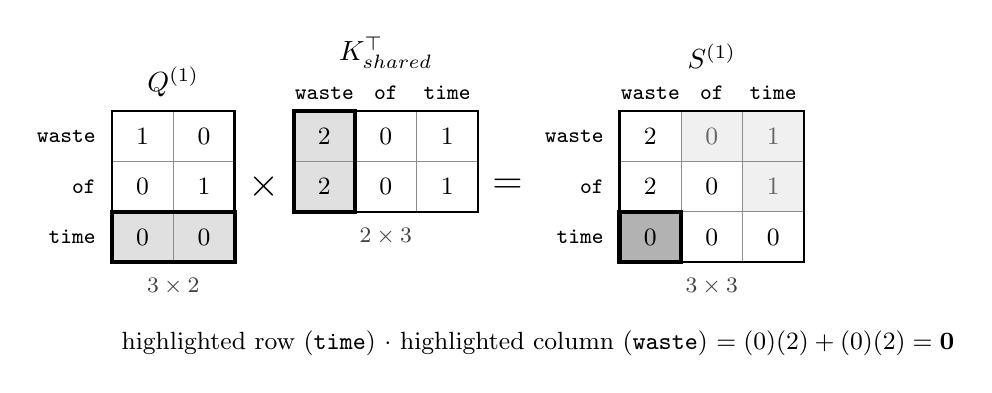
\begin{tikzpicture}
\draw[black!45, fill=white] (0.000,0.000) rectangle (0.780,-0.640);
\node[font=\small, text=black] at (0.390,-0.320) {$1$};
\draw[black!45, fill=white] (0.780,0.000) rectangle (1.560,-0.640);
\node[font=\small, text=black] at (1.170,-0.320) {$0$};
\draw[black!45, fill=white] (0.000,-0.640) rectangle (0.780,-1.279);
\node[font=\small, text=black] at (0.390,-0.959) {$0$};
\draw[black!45, fill=white] (0.780,-0.640) rectangle (1.560,-1.279);
\node[font=\small, text=black] at (1.170,-0.959) {$1$};
\draw[black!45, fill=black!12] (0.000,-1.279) rectangle (0.780,-1.919);
\node[font=\small, text=black] at (0.390,-1.599) {$0$};
\draw[black!45, fill=black!12] (0.780,-1.279) rectangle (1.560,-1.919);
\node[font=\small, text=black] at (1.170,-1.599) {$0$};
\draw[line width=1.4pt] (0.000,-1.279) rectangle (1.560,-1.919);
\draw[line width=0.9pt] (0.000,0.000) rectangle (1.560,-1.919);
\node[anchor=east, font=\footnotesize\ttfamily] at (-0.080,-0.320) {waste};
\node[anchor=east, font=\footnotesize\ttfamily] at (-0.080,-0.959) {of};
\node[anchor=east, font=\footnotesize\ttfamily] at (-0.080,-1.599) {time};
\node[anchor=south, font=\normalsize] at (0.780,0.050) {$Q^{(1)}$};
\node[anchor=north, font=\footnotesize, text=black!75] at (0.780,-1.999) {$3\times2$};
\draw[black!45, fill=black!12] (2.310,0.000) rectangle (3.090,-0.640);
\node[font=\small, text=black] at (2.700,-0.320) {$2$};
\draw[black!45, fill=white] (3.090,0.000) rectangle (3.870,-0.640);
\node[font=\small, text=black] at (3.480,-0.320) {$0$};
\draw[black!45, fill=white] (3.870,0.000) rectangle (4.650,-0.640);
\node[font=\small, text=black] at (4.260,-0.320) {$1$};
\draw[black!45, fill=black!12] (2.310,-0.640) rectangle (3.090,-1.279);
\node[font=\small, text=black] at (2.700,-0.959) {$2$};
\draw[black!45, fill=white] (3.090,-0.640) rectangle (3.870,-1.279);
\node[font=\small, text=black] at (3.480,-0.959) {$0$};
\draw[black!45, fill=white] (3.870,-0.640) rectangle (4.650,-1.279);
\node[font=\small, text=black] at (4.260,-0.959) {$1$};
\draw[line width=1.4pt] (2.310,0.000) rectangle (3.090,-1.279);
\draw[line width=0.9pt] (2.310,0.000) rectangle (4.650,-1.279);
\node[anchor=south, font=\footnotesize\ttfamily] at (2.700,0.020) {waste};
\node[anchor=south, font=\footnotesize\ttfamily] at (3.480,0.020) {of};
\node[anchor=south, font=\footnotesize\ttfamily] at (4.260,0.020) {time};
\node[anchor=south, font=\normalsize] at (3.480,0.420) {$K_{\text{shared}}^\top$};
\node[anchor=north, font=\footnotesize, text=black!75] at (3.480,-1.359) {$2\times3$};
\draw[black!45, fill=white] (6.450,0.000) rectangle (7.230,-0.640);
\node[font=\small, text=black] at (6.840,-0.320) {$2$};
\draw[black!45, fill=black!6] (7.230,0.000) rectangle (8.010,-0.640);
\node[font=\small, text=black!60] at (7.620,-0.320) {$0$};
\draw[black!45, fill=black!6] (8.010,0.000) rectangle (8.790,-0.640);
\node[font=\small, text=black!60] at (8.400,-0.320) {$1$};
\draw[black!45, fill=white] (6.450,-0.640) rectangle (7.230,-1.279);
\node[font=\small, text=black] at (6.840,-0.959) {$2$};
\draw[black!45, fill=white] (7.230,-0.640) rectangle (8.010,-1.279);
\node[font=\small, text=black] at (7.620,-0.959) {$0$};
\draw[black!45, fill=black!6] (8.010,-0.640) rectangle (8.790,-1.279);
\node[font=\small, text=black!60] at (8.400,-0.959) {$1$};
\draw[black!45, fill=black!30] (6.450,-1.279) rectangle (7.230,-1.919);
\node[font=\small, text=black] at (6.840,-1.599) {$0$};
\draw[black!45, fill=white] (7.230,-1.279) rectangle (8.010,-1.919);
\node[font=\small, text=black] at (7.620,-1.599) {$0$};
\draw[black!45, fill=white] (8.010,-1.279) rectangle (8.790,-1.919);
\node[font=\small, text=black] at (8.400,-1.599) {$0$};
\draw[line width=1.6pt] (6.450,-1.279) rectangle (7.230,-1.919);
\draw[line width=0.9pt] (6.450,0.000) rectangle (8.790,-1.919);
\node[anchor=east, font=\footnotesize\ttfamily] at (6.370,-0.320) {waste};
\node[anchor=east, font=\footnotesize\ttfamily] at (6.370,-0.959) {of};
\node[anchor=east, font=\footnotesize\ttfamily] at (6.370,-1.599) {time};
\node[anchor=south, font=\footnotesize\ttfamily] at (6.840,0.020) {waste};
\node[anchor=south, font=\footnotesize\ttfamily] at (7.620,0.020) {of};
\node[anchor=south, font=\footnotesize\ttfamily] at (8.400,0.020) {time};
\node[anchor=south, font=\normalsize] at (7.620,0.420) {$S^{(1)}$};
\node[anchor=north, font=\footnotesize, text=black!75] at (7.620,-1.999) {$3\times3$};
\node[font=\Large] at (1.935,-0.959) {$\times$};
\node[font=\Large] at (5.025,-0.959) {$=$};
\node[anchor=north west, font=\small, align=left] at (0,-2.669) {highlighted row (\texttt{time}) $\cdot$ highlighted column (\texttt{waste}) $= (0)(2) + (0)(2) = \mathbf{0}$};
\end{tikzpicture}}
\\[10pt]
\nTenFit{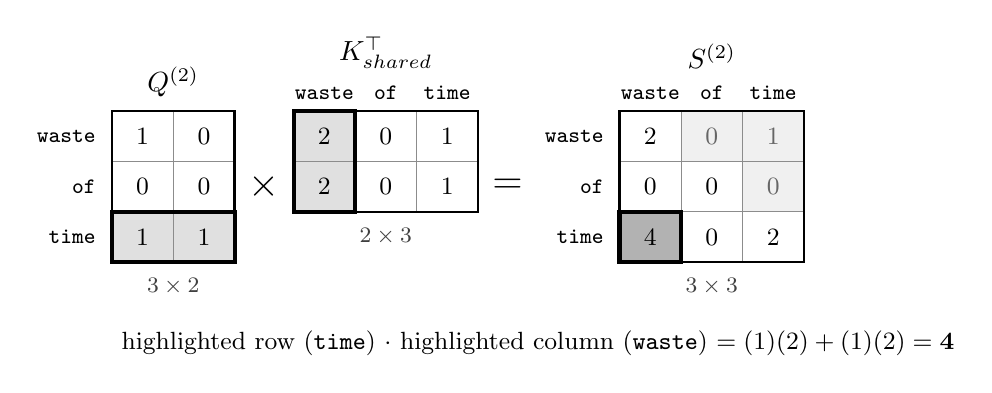
\begin{tikzpicture}
\draw[black!45, fill=white] (0.000,0.000) rectangle (0.780,-0.640);
\node[font=\small, text=black] at (0.390,-0.320) {$1$};
\draw[black!45, fill=white] (0.780,0.000) rectangle (1.560,-0.640);
\node[font=\small, text=black] at (1.170,-0.320) {$0$};
\draw[black!45, fill=white] (0.000,-0.640) rectangle (0.780,-1.279);
\node[font=\small, text=black] at (0.390,-0.959) {$0$};
\draw[black!45, fill=white] (0.780,-0.640) rectangle (1.560,-1.279);
\node[font=\small, text=black] at (1.170,-0.959) {$0$};
\draw[black!45, fill=black!12] (0.000,-1.279) rectangle (0.780,-1.919);
\node[font=\small, text=black] at (0.390,-1.599) {$1$};
\draw[black!45, fill=black!12] (0.780,-1.279) rectangle (1.560,-1.919);
\node[font=\small, text=black] at (1.170,-1.599) {$1$};
\draw[line width=1.4pt] (0.000,-1.279) rectangle (1.560,-1.919);
\draw[line width=0.9pt] (0.000,0.000) rectangle (1.560,-1.919);
\node[anchor=east, font=\footnotesize\ttfamily] at (-0.080,-0.320) {waste};
\node[anchor=east, font=\footnotesize\ttfamily] at (-0.080,-0.959) {of};
\node[anchor=east, font=\footnotesize\ttfamily] at (-0.080,-1.599) {time};
\node[anchor=south, font=\normalsize] at (0.780,0.050) {$Q^{(2)}$};
\node[anchor=north, font=\footnotesize, text=black!75] at (0.780,-1.999) {$3\times2$};
\draw[black!45, fill=black!12] (2.310,0.000) rectangle (3.090,-0.640);
\node[font=\small, text=black] at (2.700,-0.320) {$2$};
\draw[black!45, fill=white] (3.090,0.000) rectangle (3.870,-0.640);
\node[font=\small, text=black] at (3.480,-0.320) {$0$};
\draw[black!45, fill=white] (3.870,0.000) rectangle (4.650,-0.640);
\node[font=\small, text=black] at (4.260,-0.320) {$1$};
\draw[black!45, fill=black!12] (2.310,-0.640) rectangle (3.090,-1.279);
\node[font=\small, text=black] at (2.700,-0.959) {$2$};
\draw[black!45, fill=white] (3.090,-0.640) rectangle (3.870,-1.279);
\node[font=\small, text=black] at (3.480,-0.959) {$0$};
\draw[black!45, fill=white] (3.870,-0.640) rectangle (4.650,-1.279);
\node[font=\small, text=black] at (4.260,-0.959) {$1$};
\draw[line width=1.4pt] (2.310,0.000) rectangle (3.090,-1.279);
\draw[line width=0.9pt] (2.310,0.000) rectangle (4.650,-1.279);
\node[anchor=south, font=\footnotesize\ttfamily] at (2.700,0.020) {waste};
\node[anchor=south, font=\footnotesize\ttfamily] at (3.480,0.020) {of};
\node[anchor=south, font=\footnotesize\ttfamily] at (4.260,0.020) {time};
\node[anchor=south, font=\normalsize] at (3.480,0.420) {$K_{\text{shared}}^\top$};
\node[anchor=north, font=\footnotesize, text=black!75] at (3.480,-1.359) {$2\times3$};
\draw[black!45, fill=white] (6.450,0.000) rectangle (7.230,-0.640);
\node[font=\small, text=black] at (6.840,-0.320) {$2$};
\draw[black!45, fill=black!6] (7.230,0.000) rectangle (8.010,-0.640);
\node[font=\small, text=black!60] at (7.620,-0.320) {$0$};
\draw[black!45, fill=black!6] (8.010,0.000) rectangle (8.790,-0.640);
\node[font=\small, text=black!60] at (8.400,-0.320) {$1$};
\draw[black!45, fill=white] (6.450,-0.640) rectangle (7.230,-1.279);
\node[font=\small, text=black] at (6.840,-0.959) {$0$};
\draw[black!45, fill=white] (7.230,-0.640) rectangle (8.010,-1.279);
\node[font=\small, text=black] at (7.620,-0.959) {$0$};
\draw[black!45, fill=black!6] (8.010,-0.640) rectangle (8.790,-1.279);
\node[font=\small, text=black!60] at (8.400,-0.959) {$0$};
\draw[black!45, fill=black!30] (6.450,-1.279) rectangle (7.230,-1.919);
\node[font=\small, text=black] at (6.840,-1.599) {$4$};
\draw[black!45, fill=white] (7.230,-1.279) rectangle (8.010,-1.919);
\node[font=\small, text=black] at (7.620,-1.599) {$0$};
\draw[black!45, fill=white] (8.010,-1.279) rectangle (8.790,-1.919);
\node[font=\small, text=black] at (8.400,-1.599) {$2$};
\draw[line width=1.6pt] (6.450,-1.279) rectangle (7.230,-1.919);
\draw[line width=0.9pt] (6.450,0.000) rectangle (8.790,-1.919);
\node[anchor=east, font=\footnotesize\ttfamily] at (6.370,-0.320) {waste};
\node[anchor=east, font=\footnotesize\ttfamily] at (6.370,-0.959) {of};
\node[anchor=east, font=\footnotesize\ttfamily] at (6.370,-1.599) {time};
\node[anchor=south, font=\footnotesize\ttfamily] at (6.840,0.020) {waste};
\node[anchor=south, font=\footnotesize\ttfamily] at (7.620,0.020) {of};
\node[anchor=south, font=\footnotesize\ttfamily] at (8.400,0.020) {time};
\node[anchor=south, font=\normalsize] at (7.620,0.420) {$S^{(2)}$};
\node[anchor=north, font=\footnotesize, text=black!75] at (7.620,-1.999) {$3\times3$};
\node[font=\Large] at (1.935,-0.959) {$\times$};
\node[font=\Large] at (5.025,-0.959) {$=$};
\node[anchor=north west, font=\small, align=left] at (0,-2.669) {highlighted row (\texttt{time}) $\cdot$ highlighted column (\texttt{waste}) $= (1)(2) + (1)(2) = \mathbf{4}$};
\end{tikzpicture}}

\caption{Two query heads, one shared key head, real toy numbers. Same keys, different questions: for
\tok{time} looking at \tok{waste}, head 1 scores \nTenFigSOneTW\ and head 2 scores \nTenFigSTwoTW.
Grey cells are hidden by the causal mask.}
\end{figure}

Sharing keys does not make the heads agree, because each head still multiplies the shared keys by its own
questions. Head 1's query for \tok{time} is $(0,0)$: in this head, \tok{time} asks nothing at all. What is
shared is the \emph{storage}: one key head to keep in the cache instead of two.

\begin{wrongidea}{10.6}
``Number of heads times head width must equal the model width.'' It does in the original transformer and in GPT-2,
which is why it looks like a rule. It is a choice. The residual stream must keep width $d$, and $W_O$ guarantees
that whatever the heads produce is brought back to $d$. Qwen3-0.6B spends more numbers on asking (2{,}048) than it
keeps in the stream (1{,}024).
\end{wrongidea}

\paragraph{Two more changes inside attention.} Qwen3 normalises every query and every key before the dot product
(\emph{QK-norm}; Henry et al., 2020; Yang et al., 2025). Remember the two knobs of \S3.2: direction and
length. QK-norm fixes the length knob, so scores cannot grow without limit as training goes on; the model has to
express agreement mostly through direction. And positions enter by rotating queries and keys (RoPE, Chapter 4)
instead of GPT-2's learned table of 1{,}024 position vectors.

\begin{wrongidea}{10.2}
``More attention heads always help.'' It is tempting because each head asks its own question, so more heads
sound like more questions. But heads split a
fixed budget of numbers into more, narrower questions. Narrower heads describe each token with fewer numbers.
Qwen3 chose 16 query heads but only 8 key-value heads; the right count is something to test, not assume
(Chapter 11).
\end{wrongidea}

\begin{checkq}
In Qwen3-0.6B, what shape is the output projection $W_O$ of one layer?
\begin{options}
\item $1{,}024\times1{,}024$, because heads times width must equal $d$.
\item $2{,}048\times1{,}024$, from the 16 query heads back to the stream width.
\item $1{,}024\times2{,}048$, because outputs are wider than inputs.
\item It has no $W_O$; the heads are added straight into the stream.
\end{options}
\end{checkq}

\Summary{Qwen3 asks with 16 heads of 128 numbers, shares 8 key-value heads, fixes query and key lengths, and
rotates them for position; $W_O$ brings everything back to the stream width.}

%---------------------------------------------------------------------
\subsection*{10.4\quad Counting every parameter, then checking}

Before counting, look. Figure~\ref{fig:ch10scale} draws every weight matrix of one block to the same scale,
with the shapes read from the reference code library's own model classes. Each rectangle has one row per input
number and one column per output number, so its area is its parameter count.

\begin{figure}[!htb]
\centering
% AUTO-GENERATED by code/figlib.py helpers -- do not edit
\nTenFit{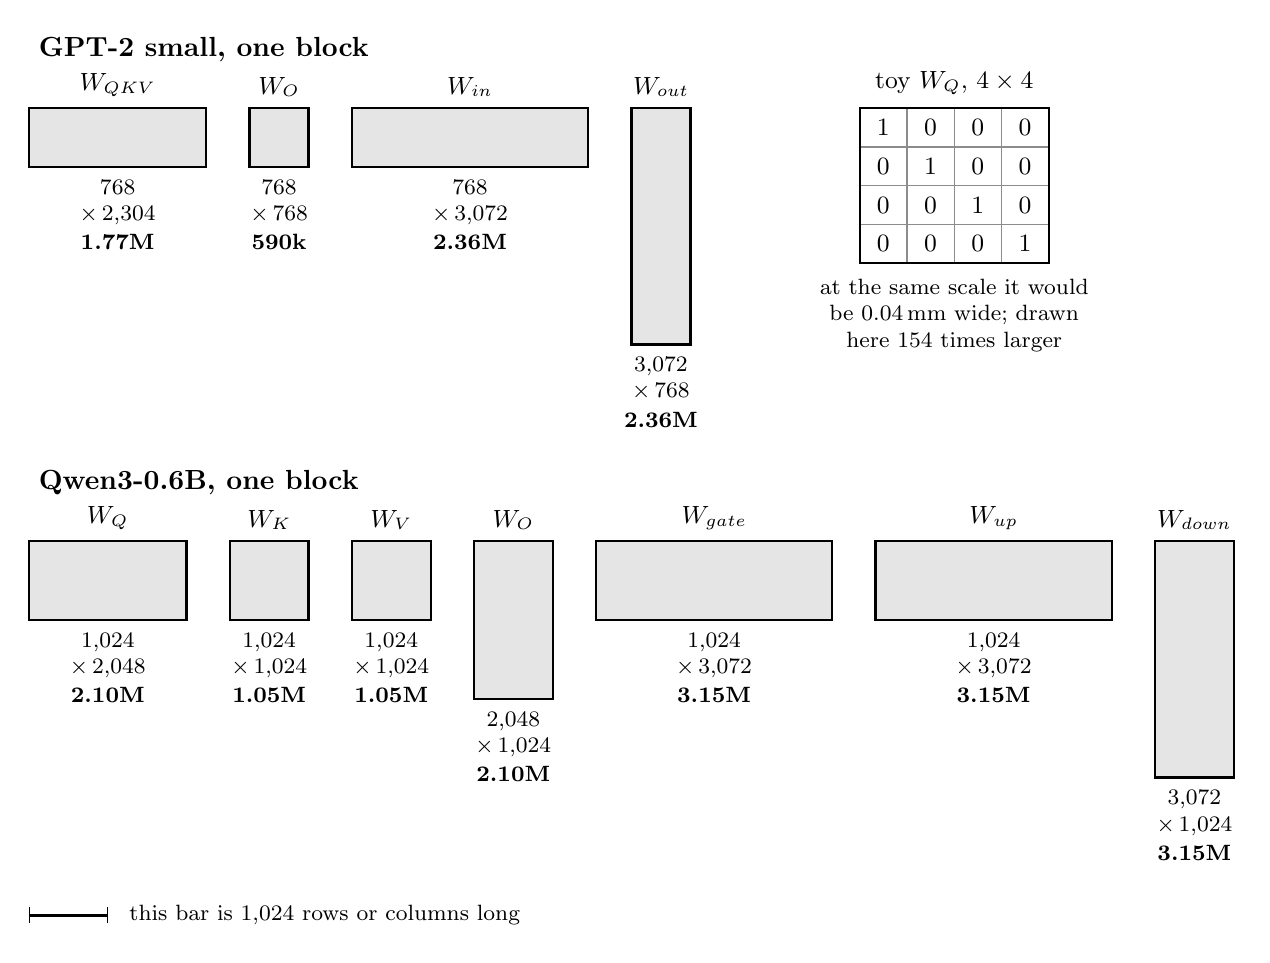
\begin{tikzpicture}
\node[anchor=west, font=\normalsize\bfseries] at (0,0.75) {GPT-2 small, one block};
\draw[line width=0.8pt, fill=black!10] (0.000,0.000) rectangle (2.250,-0.750);
\node[anchor=south, font=\small] at (1.125,0.020) {$W_{QKV}$};
\node[anchor=north, font=\footnotesize, align=center] at (1.125,-0.790) {768\\$\times$\,2{,}304\\[1pt]\textbf{1.77M}};
\draw[line width=0.8pt, fill=black!10] (2.800,0.000) rectangle (3.550,-0.750);
\node[anchor=south, font=\small] at (3.175,0.020) {$W_O$};
\node[anchor=north, font=\footnotesize, align=center] at (3.175,-0.790) {768\\$\times$\,768\\[1pt]\textbf{590k}};
\draw[line width=0.8pt, fill=black!10] (4.100,0.000) rectangle (7.100,-0.750);
\node[anchor=south, font=\small] at (5.600,0.020) {$W_{\text{in}}$};
\node[anchor=north, font=\footnotesize, align=center] at (5.600,-0.790) {768\\$\times$\,3{,}072\\[1pt]\textbf{2.36M}};
\draw[line width=0.8pt, fill=black!10] (7.650,0.000) rectangle (8.400,-3.000);
\node[anchor=south, font=\small] at (8.025,0.020) {$W_{\text{out}}$};
\node[anchor=north, font=\footnotesize, align=center] at (8.025,-3.040) {3{,}072\\$\times$\,768\\[1pt]\textbf{2.36M}};
\draw[black!45, fill=white] (10.550,0.000) rectangle (11.150,-0.492);
\node[font=\small, text=black] at (10.850,-0.246) {$1$};
\draw[black!45, fill=white] (11.150,0.000) rectangle (11.750,-0.492);
\node[font=\small, text=black] at (11.450,-0.246) {$0$};
\draw[black!45, fill=white] (11.750,0.000) rectangle (12.350,-0.492);
\node[font=\small, text=black] at (12.050,-0.246) {$0$};
\draw[black!45, fill=white] (12.350,0.000) rectangle (12.950,-0.492);
\node[font=\small, text=black] at (12.650,-0.246) {$0$};
\draw[black!45, fill=white] (10.550,-0.492) rectangle (11.150,-0.984);
\node[font=\small, text=black] at (10.850,-0.738) {$0$};
\draw[black!45, fill=white] (11.150,-0.492) rectangle (11.750,-0.984);
\node[font=\small, text=black] at (11.450,-0.738) {$1$};
\draw[black!45, fill=white] (11.750,-0.492) rectangle (12.350,-0.984);
\node[font=\small, text=black] at (12.050,-0.738) {$0$};
\draw[black!45, fill=white] (12.350,-0.492) rectangle (12.950,-0.984);
\node[font=\small, text=black] at (12.650,-0.738) {$0$};
\draw[black!45, fill=white] (10.550,-0.984) rectangle (11.150,-1.476);
\node[font=\small, text=black] at (10.850,-1.230) {$0$};
\draw[black!45, fill=white] (11.150,-0.984) rectangle (11.750,-1.476);
\node[font=\small, text=black] at (11.450,-1.230) {$0$};
\draw[black!45, fill=white] (11.750,-0.984) rectangle (12.350,-1.476);
\node[font=\small, text=black] at (12.050,-1.230) {$1$};
\draw[black!45, fill=white] (12.350,-0.984) rectangle (12.950,-1.476);
\node[font=\small, text=black] at (12.650,-1.230) {$0$};
\draw[black!45, fill=white] (10.550,-1.476) rectangle (11.150,-1.968);
\node[font=\small, text=black] at (10.850,-1.722) {$0$};
\draw[black!45, fill=white] (11.150,-1.476) rectangle (11.750,-1.968);
\node[font=\small, text=black] at (11.450,-1.722) {$0$};
\draw[black!45, fill=white] (11.750,-1.476) rectangle (12.350,-1.968);
\node[font=\small, text=black] at (12.050,-1.722) {$0$};
\draw[black!45, fill=white] (12.350,-1.476) rectangle (12.950,-1.968);
\node[font=\small, text=black] at (12.650,-1.722) {$1$};
\draw[line width=0.9pt] (10.550,0.000) rectangle (12.950,-1.968);
\node[anchor=south, font=\small, align=center] at (11.750,0.05) {toy $W_Q$, $4\times4$};
\node[anchor=north, font=\footnotesize, align=center, text width=4.6cm] at (11.750,-2.048) {at the same scale it would be 0.04\,mm wide; drawn here 154 times larger};
\node[anchor=west, font=\normalsize\bfseries] at (0,-4.75) {Qwen3-0.6B, one block};
\draw[line width=0.8pt, fill=black!10] (0.000,-5.500) rectangle (2.000,-6.500);
\node[anchor=south, font=\small] at (1.000,-5.480) {$W_Q$};
\node[anchor=north, font=\footnotesize, align=center] at (1.000,-6.540) {1{,}024\\$\times$\,2{,}048\\[1pt]\textbf{2.10M}};
\draw[line width=0.8pt, fill=black!10] (2.550,-5.500) rectangle (3.550,-6.500);
\node[anchor=south, font=\small] at (3.050,-5.480) {$W_K$};
\node[anchor=north, font=\footnotesize, align=center] at (3.050,-6.540) {1{,}024\\$\times$\,1{,}024\\[1pt]\textbf{1.05M}};
\draw[line width=0.8pt, fill=black!10] (4.100,-5.500) rectangle (5.100,-6.500);
\node[anchor=south, font=\small] at (4.600,-5.480) {$W_V$};
\node[anchor=north, font=\footnotesize, align=center] at (4.600,-6.540) {1{,}024\\$\times$\,1{,}024\\[1pt]\textbf{1.05M}};
\draw[line width=0.8pt, fill=black!10] (5.650,-5.500) rectangle (6.650,-7.500);
\node[anchor=south, font=\small] at (6.150,-5.480) {$W_O$};
\node[anchor=north, font=\footnotesize, align=center] at (6.150,-7.540) {2{,}048\\$\times$\,1{,}024\\[1pt]\textbf{2.10M}};
\draw[line width=0.8pt, fill=black!10] (7.200,-5.500) rectangle (10.200,-6.500);
\node[anchor=south, font=\small] at (8.700,-5.480) {$W_{\text{gate}}$};
\node[anchor=north, font=\footnotesize, align=center] at (8.700,-6.540) {1{,}024\\$\times$\,3{,}072\\[1pt]\textbf{3.15M}};
\draw[line width=0.8pt, fill=black!10] (10.750,-5.500) rectangle (13.750,-6.500);
\node[anchor=south, font=\small] at (12.250,-5.480) {$W_{\text{up}}$};
\node[anchor=north, font=\footnotesize, align=center] at (12.250,-6.540) {1{,}024\\$\times$\,3{,}072\\[1pt]\textbf{3.15M}};
\draw[line width=0.8pt, fill=black!10] (14.300,-5.500) rectangle (15.300,-8.500);
\node[anchor=south, font=\small] at (14.800,-5.480) {$W_{\text{down}}$};
\node[anchor=north, font=\footnotesize, align=center] at (14.800,-8.540) {3{,}072\\$\times$\,1{,}024\\[1pt]\textbf{3.15M}};
\draw[line width=1pt] (0,-10.25) -- (1,-10.25); \draw (0,-10.15) -- (0,-10.35) (1,-10.15) -- (1,-10.35); \node[anchor=west, font=\footnotesize] at (1.15,-10.25) {this bar is 1{,}024 rows or columns long};
\end{tikzpicture}}

\caption{One block's weight matrices, drawn to scale (the bar at the bottom left is 1{,}024 rows or columns long). Under each: rows
$\times$ columns and the count in millions (M). Notice how much of the area the three MLP matrices on the right
take, and that the toy's whole query matrix would be a dot.}
\label{fig:ch10scale}
\end{figure}

Now count. Each component's count follows from its shape:
\begin{itemize}
\item embedding table: vocabulary $\times\ d$; GPT-2 adds a position table, $1{,}024\times d$;
\item attention: $W_Q$, $W_K$, $W_V$, $W_O$ (GPT-2 also has a bias for every output number); Qwen3 adds two
QK-norm scales of 128;
\item MLP: GPT-2 has two matrices, $d\times3{,}072$ and $3{,}072\times d$, plus biases; Qwen3's SwiGLU
(Shazeer, 2020) has three, a gate, an up and a down matrix;
\item norms: a LayerNorm has a scale and a shift for each of the $d$ numbers ($2d$); an RMSNorm has only
the scale ($d$). Two per block, one at the end;
\item unembedding: both models reuse the embedding table (\emph{tied} weights, Chapter 7), so it adds nothing.
\end{itemize}

\paragraph{SwiGLU on the toy.} Qwen3's MLP has three matrices where GPT-2's has two. Two of them read the
same input: $W_{\text{up}}$ proposes values, and $W_{\text{gate}}$ decides, entry by entry, how much of each
value gets through. \Predict If a gate entry is negative, does its value get through, get flipped, or get
mostly stopped? Below, \tok{time}'s attention output from Chapter 3, $\bm{x}=\nTenFigX$, goes through a
pencil-sized SwiGLU (inner width 4, weights chosen by hand).

\begin{figure}[!htb]
\centering
% AUTO-GENERATED by code/figlib.py helpers -- do not edit
\nTenFit{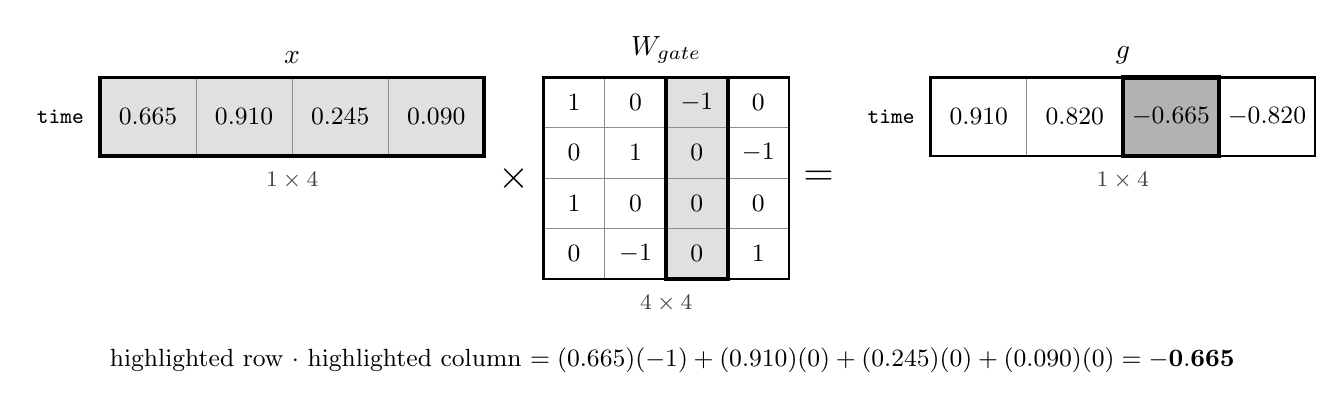
\begin{tikzpicture}
\draw[black!45, fill=black!12] (0.000,0.000) rectangle (1.220,-1.000);
\node[font=\small, text=black] at (0.610,-0.500) {$0.665$};
\draw[black!45, fill=black!12] (1.220,0.000) rectangle (2.440,-1.000);
\node[font=\small, text=black] at (1.830,-0.500) {$0.910$};
\draw[black!45, fill=black!12] (2.440,0.000) rectangle (3.660,-1.000);
\node[font=\small, text=black] at (3.050,-0.500) {$0.245$};
\draw[black!45, fill=black!12] (3.660,0.000) rectangle (4.880,-1.000);
\node[font=\small, text=black] at (4.270,-0.500) {$0.090$};
\draw[line width=1.4pt] (0.000,0.000) rectangle (4.880,-1.000);
\draw[line width=0.9pt] (0.000,0.000) rectangle (4.880,-1.000);
\node[anchor=east, font=\footnotesize\ttfamily] at (-0.080,-0.500) {time};
\node[anchor=south, font=\normalsize] at (2.440,0.050) {$\bm{x}$};
\node[anchor=north, font=\footnotesize, text=black!75] at (2.440,-1.080) {$1\times4$};
\draw[black!45, fill=white] (5.630,0.000) rectangle (6.410,-0.640);
\node[font=\small, text=black] at (6.020,-0.320) {$1$};
\draw[black!45, fill=white] (6.410,0.000) rectangle (7.190,-0.640);
\node[font=\small, text=black] at (6.800,-0.320) {$0$};
\draw[black!45, fill=black!12] (7.190,0.000) rectangle (7.970,-0.640);
\node[font=\small, text=black] at (7.580,-0.320) {$-1$};
\draw[black!45, fill=white] (7.970,0.000) rectangle (8.750,-0.640);
\node[font=\small, text=black] at (8.360,-0.320) {$0$};
\draw[black!45, fill=white] (5.630,-0.640) rectangle (6.410,-1.279);
\node[font=\small, text=black] at (6.020,-0.959) {$0$};
\draw[black!45, fill=white] (6.410,-0.640) rectangle (7.190,-1.279);
\node[font=\small, text=black] at (6.800,-0.959) {$1$};
\draw[black!45, fill=black!12] (7.190,-0.640) rectangle (7.970,-1.279);
\node[font=\small, text=black] at (7.580,-0.959) {$0$};
\draw[black!45, fill=white] (7.970,-0.640) rectangle (8.750,-1.279);
\node[font=\small, text=black] at (8.360,-0.959) {$-1$};
\draw[black!45, fill=white] (5.630,-1.279) rectangle (6.410,-1.919);
\node[font=\small, text=black] at (6.020,-1.599) {$1$};
\draw[black!45, fill=white] (6.410,-1.279) rectangle (7.190,-1.919);
\node[font=\small, text=black] at (6.800,-1.599) {$0$};
\draw[black!45, fill=black!12] (7.190,-1.279) rectangle (7.970,-1.919);
\node[font=\small, text=black] at (7.580,-1.599) {$0$};
\draw[black!45, fill=white] (7.970,-1.279) rectangle (8.750,-1.919);
\node[font=\small, text=black] at (8.360,-1.599) {$0$};
\draw[black!45, fill=white] (5.630,-1.919) rectangle (6.410,-2.558);
\node[font=\small, text=black] at (6.020,-2.239) {$0$};
\draw[black!45, fill=white] (6.410,-1.919) rectangle (7.190,-2.558);
\node[font=\small, text=black] at (6.800,-2.239) {$-1$};
\draw[black!45, fill=black!12] (7.190,-1.919) rectangle (7.970,-2.558);
\node[font=\small, text=black] at (7.580,-2.239) {$0$};
\draw[black!45, fill=white] (7.970,-1.919) rectangle (8.750,-2.558);
\node[font=\small, text=black] at (8.360,-2.239) {$1$};
\draw[line width=1.4pt] (7.190,0.000) rectangle (7.970,-2.558);
\draw[line width=0.9pt] (5.630,0.000) rectangle (8.750,-2.558);
\node[anchor=south, font=\normalsize] at (7.190,0.050) {$W_{\text{gate}}$};
\node[anchor=north, font=\footnotesize, text=black!75] at (7.190,-2.638) {$4\times4$};
\draw[black!45, fill=white] (10.550,0.000) rectangle (11.770,-1.000);
\node[font=\small, text=black] at (11.160,-0.500) {$0.910$};
\draw[black!45, fill=white] (11.770,0.000) rectangle (12.990,-1.000);
\node[font=\small, text=black] at (12.380,-0.500) {$0.820$};
\draw[black!45, fill=black!30] (12.990,0.000) rectangle (14.210,-1.000);
\node[font=\small, text=black] at (13.600,-0.500) {$-0.665$};
\draw[black!45, fill=white] (14.210,0.000) rectangle (15.430,-1.000);
\node[font=\small, text=black] at (14.820,-0.500) {$-0.820$};
\draw[line width=1.6pt] (12.990,0.000) rectangle (14.210,-1.000);
\draw[line width=0.9pt] (10.550,0.000) rectangle (15.430,-1.000);
\node[anchor=east, font=\footnotesize\ttfamily] at (10.470,-0.500) {time};
\node[anchor=south, font=\normalsize] at (12.990,0.050) {$\bm{g}$};
\node[anchor=north, font=\footnotesize, text=black!75] at (12.990,-1.080) {$1\times4$};
\node[font=\Large] at (5.255,-1.279) {$\times$};
\node[font=\Large] at (9.125,-1.279) {$=$};
\node[anchor=north west, font=\small] at (0,-3.308) {highlighted row $\cdot$ highlighted column $= (0.665)(-1) + (0.910)(0) + (0.245)(0) + (0.090)(0) = \mathbf{-0.665}$};
\end{tikzpicture}}
\\[10pt]
\nTenFit{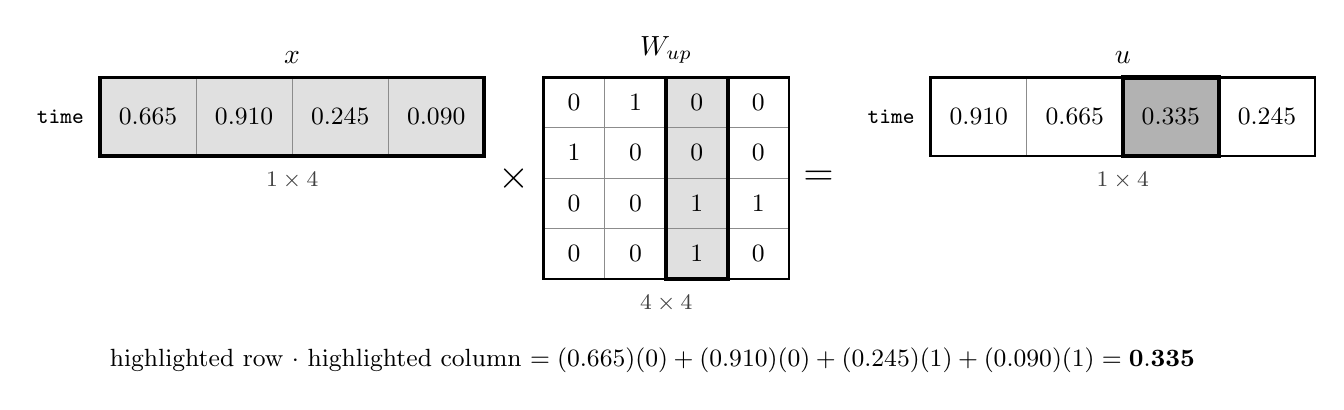
\begin{tikzpicture}
\draw[black!45, fill=black!12] (0.000,0.000) rectangle (1.220,-1.000);
\node[font=\small, text=black] at (0.610,-0.500) {$0.665$};
\draw[black!45, fill=black!12] (1.220,0.000) rectangle (2.440,-1.000);
\node[font=\small, text=black] at (1.830,-0.500) {$0.910$};
\draw[black!45, fill=black!12] (2.440,0.000) rectangle (3.660,-1.000);
\node[font=\small, text=black] at (3.050,-0.500) {$0.245$};
\draw[black!45, fill=black!12] (3.660,0.000) rectangle (4.880,-1.000);
\node[font=\small, text=black] at (4.270,-0.500) {$0.090$};
\draw[line width=1.4pt] (0.000,0.000) rectangle (4.880,-1.000);
\draw[line width=0.9pt] (0.000,0.000) rectangle (4.880,-1.000);
\node[anchor=east, font=\footnotesize\ttfamily] at (-0.080,-0.500) {time};
\node[anchor=south, font=\normalsize] at (2.440,0.050) {$\bm{x}$};
\node[anchor=north, font=\footnotesize, text=black!75] at (2.440,-1.080) {$1\times4$};
\draw[black!45, fill=white] (5.630,0.000) rectangle (6.410,-0.640);
\node[font=\small, text=black] at (6.020,-0.320) {$0$};
\draw[black!45, fill=white] (6.410,0.000) rectangle (7.190,-0.640);
\node[font=\small, text=black] at (6.800,-0.320) {$1$};
\draw[black!45, fill=black!12] (7.190,0.000) rectangle (7.970,-0.640);
\node[font=\small, text=black] at (7.580,-0.320) {$0$};
\draw[black!45, fill=white] (7.970,0.000) rectangle (8.750,-0.640);
\node[font=\small, text=black] at (8.360,-0.320) {$0$};
\draw[black!45, fill=white] (5.630,-0.640) rectangle (6.410,-1.279);
\node[font=\small, text=black] at (6.020,-0.959) {$1$};
\draw[black!45, fill=white] (6.410,-0.640) rectangle (7.190,-1.279);
\node[font=\small, text=black] at (6.800,-0.959) {$0$};
\draw[black!45, fill=black!12] (7.190,-0.640) rectangle (7.970,-1.279);
\node[font=\small, text=black] at (7.580,-0.959) {$0$};
\draw[black!45, fill=white] (7.970,-0.640) rectangle (8.750,-1.279);
\node[font=\small, text=black] at (8.360,-0.959) {$0$};
\draw[black!45, fill=white] (5.630,-1.279) rectangle (6.410,-1.919);
\node[font=\small, text=black] at (6.020,-1.599) {$0$};
\draw[black!45, fill=white] (6.410,-1.279) rectangle (7.190,-1.919);
\node[font=\small, text=black] at (6.800,-1.599) {$0$};
\draw[black!45, fill=black!12] (7.190,-1.279) rectangle (7.970,-1.919);
\node[font=\small, text=black] at (7.580,-1.599) {$1$};
\draw[black!45, fill=white] (7.970,-1.279) rectangle (8.750,-1.919);
\node[font=\small, text=black] at (8.360,-1.599) {$1$};
\draw[black!45, fill=white] (5.630,-1.919) rectangle (6.410,-2.558);
\node[font=\small, text=black] at (6.020,-2.239) {$0$};
\draw[black!45, fill=white] (6.410,-1.919) rectangle (7.190,-2.558);
\node[font=\small, text=black] at (6.800,-2.239) {$0$};
\draw[black!45, fill=black!12] (7.190,-1.919) rectangle (7.970,-2.558);
\node[font=\small, text=black] at (7.580,-2.239) {$1$};
\draw[black!45, fill=white] (7.970,-1.919) rectangle (8.750,-2.558);
\node[font=\small, text=black] at (8.360,-2.239) {$0$};
\draw[line width=1.4pt] (7.190,0.000) rectangle (7.970,-2.558);
\draw[line width=0.9pt] (5.630,0.000) rectangle (8.750,-2.558);
\node[anchor=south, font=\normalsize] at (7.190,0.050) {$W_{\text{up}}$};
\node[anchor=north, font=\footnotesize, text=black!75] at (7.190,-2.638) {$4\times4$};
\draw[black!45, fill=white] (10.550,0.000) rectangle (11.770,-1.000);
\node[font=\small, text=black] at (11.160,-0.500) {$0.910$};
\draw[black!45, fill=white] (11.770,0.000) rectangle (12.990,-1.000);
\node[font=\small, text=black] at (12.380,-0.500) {$0.665$};
\draw[black!45, fill=black!30] (12.990,0.000) rectangle (14.210,-1.000);
\node[font=\small, text=black] at (13.600,-0.500) {$0.335$};
\draw[black!45, fill=white] (14.210,0.000) rectangle (15.430,-1.000);
\node[font=\small, text=black] at (14.820,-0.500) {$0.245$};
\draw[line width=1.6pt] (12.990,0.000) rectangle (14.210,-1.000);
\draw[line width=0.9pt] (10.550,0.000) rectangle (15.430,-1.000);
\node[anchor=east, font=\footnotesize\ttfamily] at (10.470,-0.500) {time};
\node[anchor=south, font=\normalsize] at (12.990,0.050) {$\bm{u}$};
\node[anchor=north, font=\footnotesize, text=black!75] at (12.990,-1.080) {$1\times4$};
\node[font=\Large] at (5.255,-1.279) {$\times$};
\node[font=\Large] at (9.125,-1.279) {$=$};
\node[anchor=north west, font=\small] at (0,-3.308) {highlighted row $\cdot$ highlighted column $= (0.665)(0) + (0.910)(0) + (0.245)(1) + (0.090)(1) = \mathbf{0.335}$};
\end{tikzpicture}}
\\[10pt]
\nTenFit{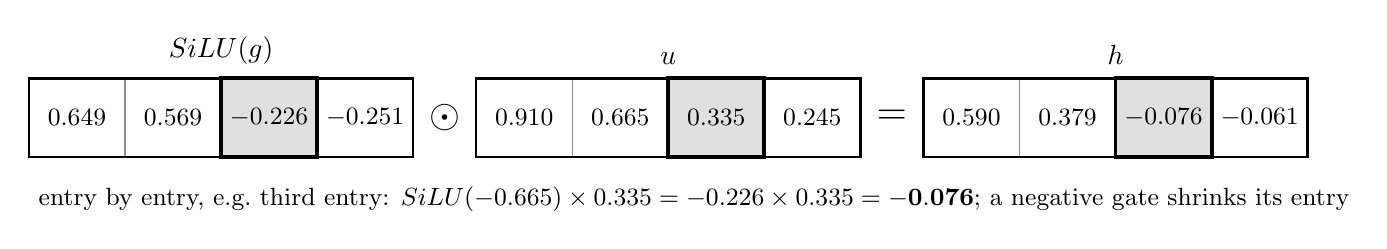
\begin{tikzpicture}
\draw[black!45, fill=white] (0.000,0.000) rectangle (1.220,-1.000);
\node[font=\small, text=black] at (0.610,-0.500) {$0.649$};
\draw[black!45, fill=white] (1.220,0.000) rectangle (2.440,-1.000);
\node[font=\small, text=black] at (1.830,-0.500) {$0.569$};
\draw[black!45, fill=black!12] (2.440,0.000) rectangle (3.660,-1.000);
\node[font=\small, text=black] at (3.050,-0.500) {$-0.226$};
\draw[black!45, fill=white] (3.660,0.000) rectangle (4.880,-1.000);
\node[font=\small, text=black] at (4.270,-0.500) {$-0.251$};
\draw[line width=1.4pt] (2.440,0.000) rectangle (3.660,-1.000);
\draw[line width=0.9pt] (0.000,0.000) rectangle (4.880,-1.000);
\node[anchor=south, font=\normalsize] at (2.440,0.050) {$\operatorname{SiLU}(\bm{g})$};
\node[font=\Large] at (5.280,-0.500) {$\odot$};
\draw[black!45, fill=white] (5.680,0.000) rectangle (6.900,-1.000);
\node[font=\small, text=black] at (6.290,-0.500) {$0.910$};
\draw[black!45, fill=white] (6.900,0.000) rectangle (8.120,-1.000);
\node[font=\small, text=black] at (7.510,-0.500) {$0.665$};
\draw[black!45, fill=black!12] (8.120,0.000) rectangle (9.340,-1.000);
\node[font=\small, text=black] at (8.730,-0.500) {$0.335$};
\draw[black!45, fill=white] (9.340,0.000) rectangle (10.560,-1.000);
\node[font=\small, text=black] at (9.950,-0.500) {$0.245$};
\draw[line width=1.4pt] (8.120,0.000) rectangle (9.340,-1.000);
\draw[line width=0.9pt] (5.680,0.000) rectangle (10.560,-1.000);
\node[anchor=south, font=\normalsize] at (8.120,0.050) {$\bm{u}$};
\node[font=\Large] at (10.960,-0.500) {$=$};
\draw[black!45, fill=white] (11.360,0.000) rectangle (12.580,-1.000);
\node[font=\small, text=black] at (11.970,-0.500) {$0.590$};
\draw[black!45, fill=white] (12.580,0.000) rectangle (13.800,-1.000);
\node[font=\small, text=black] at (13.190,-0.500) {$0.379$};
\draw[black!45, fill=black!12] (13.800,0.000) rectangle (15.020,-1.000);
\node[font=\small, text=black] at (14.410,-0.500) {$-0.076$};
\draw[black!45, fill=white] (15.020,0.000) rectangle (16.240,-1.000);
\node[font=\small, text=black] at (15.630,-0.500) {$-0.061$};
\draw[line width=1.4pt] (13.800,0.000) rectangle (15.020,-1.000);
\draw[line width=0.9pt] (11.360,0.000) rectangle (16.240,-1.000);
\node[anchor=south, font=\normalsize] at (13.800,0.050) {$\bm{h}$};
\node[anchor=north west, font=\small] at (0,-1.25) {entry by entry, e.g.\ third entry: $\operatorname{SiLU}(-0.665) \times 0.335 = -0.226\times0.335 = \mathbf{-0.076}$; a negative gate shrinks its entry};
\end{tikzpicture}}
\\[10pt]
\nTenFit{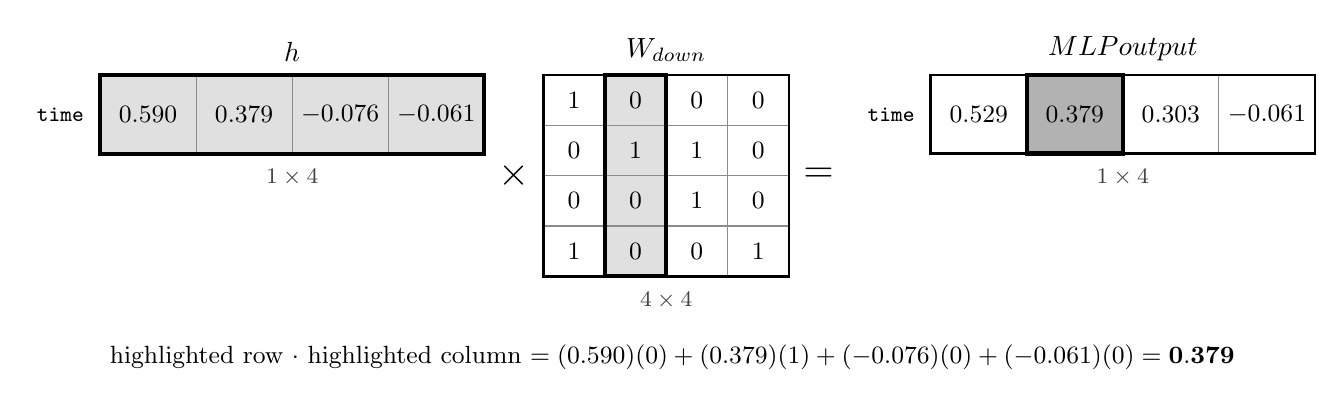
\begin{tikzpicture}
\draw[black!45, fill=black!12] (0.000,0.000) rectangle (1.220,-1.000);
\node[font=\small, text=black] at (0.610,-0.500) {$0.590$};
\draw[black!45, fill=black!12] (1.220,0.000) rectangle (2.440,-1.000);
\node[font=\small, text=black] at (1.830,-0.500) {$0.379$};
\draw[black!45, fill=black!12] (2.440,0.000) rectangle (3.660,-1.000);
\node[font=\small, text=black] at (3.050,-0.500) {$-0.076$};
\draw[black!45, fill=black!12] (3.660,0.000) rectangle (4.880,-1.000);
\node[font=\small, text=black] at (4.270,-0.500) {$-0.061$};
\draw[line width=1.4pt] (0.000,0.000) rectangle (4.880,-1.000);
\draw[line width=0.9pt] (0.000,0.000) rectangle (4.880,-1.000);
\node[anchor=east, font=\footnotesize\ttfamily] at (-0.080,-0.500) {time};
\node[anchor=south, font=\normalsize] at (2.440,0.050) {$\bm{h}$};
\node[anchor=north, font=\footnotesize, text=black!75] at (2.440,-1.080) {$1\times4$};
\draw[black!45, fill=white] (5.630,0.000) rectangle (6.410,-0.640);
\node[font=\small, text=black] at (6.020,-0.320) {$1$};
\draw[black!45, fill=black!12] (6.410,0.000) rectangle (7.190,-0.640);
\node[font=\small, text=black] at (6.800,-0.320) {$0$};
\draw[black!45, fill=white] (7.190,0.000) rectangle (7.970,-0.640);
\node[font=\small, text=black] at (7.580,-0.320) {$0$};
\draw[black!45, fill=white] (7.970,0.000) rectangle (8.750,-0.640);
\node[font=\small, text=black] at (8.360,-0.320) {$0$};
\draw[black!45, fill=white] (5.630,-0.640) rectangle (6.410,-1.279);
\node[font=\small, text=black] at (6.020,-0.959) {$0$};
\draw[black!45, fill=black!12] (6.410,-0.640) rectangle (7.190,-1.279);
\node[font=\small, text=black] at (6.800,-0.959) {$1$};
\draw[black!45, fill=white] (7.190,-0.640) rectangle (7.970,-1.279);
\node[font=\small, text=black] at (7.580,-0.959) {$1$};
\draw[black!45, fill=white] (7.970,-0.640) rectangle (8.750,-1.279);
\node[font=\small, text=black] at (8.360,-0.959) {$0$};
\draw[black!45, fill=white] (5.630,-1.279) rectangle (6.410,-1.919);
\node[font=\small, text=black] at (6.020,-1.599) {$0$};
\draw[black!45, fill=black!12] (6.410,-1.279) rectangle (7.190,-1.919);
\node[font=\small, text=black] at (6.800,-1.599) {$0$};
\draw[black!45, fill=white] (7.190,-1.279) rectangle (7.970,-1.919);
\node[font=\small, text=black] at (7.580,-1.599) {$1$};
\draw[black!45, fill=white] (7.970,-1.279) rectangle (8.750,-1.919);
\node[font=\small, text=black] at (8.360,-1.599) {$0$};
\draw[black!45, fill=white] (5.630,-1.919) rectangle (6.410,-2.558);
\node[font=\small, text=black] at (6.020,-2.239) {$1$};
\draw[black!45, fill=black!12] (6.410,-1.919) rectangle (7.190,-2.558);
\node[font=\small, text=black] at (6.800,-2.239) {$0$};
\draw[black!45, fill=white] (7.190,-1.919) rectangle (7.970,-2.558);
\node[font=\small, text=black] at (7.580,-2.239) {$0$};
\draw[black!45, fill=white] (7.970,-1.919) rectangle (8.750,-2.558);
\node[font=\small, text=black] at (8.360,-2.239) {$1$};
\draw[line width=1.4pt] (6.410,0.000) rectangle (7.190,-2.558);
\draw[line width=0.9pt] (5.630,0.000) rectangle (8.750,-2.558);
\node[anchor=south, font=\normalsize] at (7.190,0.050) {$W_{\text{down}}$};
\node[anchor=north, font=\footnotesize, text=black!75] at (7.190,-2.638) {$4\times4$};
\draw[black!45, fill=white] (10.550,0.000) rectangle (11.770,-1.000);
\node[font=\small, text=black] at (11.160,-0.500) {$0.529$};
\draw[black!45, fill=black!30] (11.770,0.000) rectangle (12.990,-1.000);
\node[font=\small, text=black] at (12.380,-0.500) {$0.379$};
\draw[black!45, fill=white] (12.990,0.000) rectangle (14.210,-1.000);
\node[font=\small, text=black] at (13.600,-0.500) {$0.303$};
\draw[black!45, fill=white] (14.210,0.000) rectangle (15.430,-1.000);
\node[font=\small, text=black] at (14.820,-0.500) {$-0.061$};
\draw[line width=1.6pt] (11.770,0.000) rectangle (12.990,-1.000);
\draw[line width=0.9pt] (10.550,0.000) rectangle (15.430,-1.000);
\node[anchor=east, font=\footnotesize\ttfamily] at (10.470,-0.500) {time};
\node[anchor=south, font=\normalsize] at (12.990,0.050) {$\text{MLP output}$};
\node[anchor=north, font=\footnotesize, text=black!75] at (12.990,-1.080) {$1\times4$};
\node[font=\Large] at (5.255,-1.279) {$\times$};
\node[font=\Large] at (9.125,-1.279) {$=$};
\node[anchor=north west, font=\small] at (0,-3.308) {highlighted row $\cdot$ highlighted column $= (0.590)(0) + (0.379)(1) + (-0.076)(0) + (-0.061)(0) = \mathbf{0.379}$};
\end{tikzpicture}}

\caption{SwiGLU with real numbers. Gate and up are two matrix products of the same vector; $\operatorname{SiLU}(g)
= g/(1+e^{-g})$ squashes the gate (close to $g$ when $g$ is large, close to 0 when $g$ is very negative); the
two are multiplied entry by entry ($\odot$); $W_{\text{down}}$ brings the result back to width $d$. Output:
$\nTenFigY$.}
\end{figure}

\Sanity The third gate entry is negative, and its entry of $\bm{h}$ comes out small and of the opposite sign.
A gate is a dial on each value, which a plain MLP (Chapter 5) does not have; that is the whole idea, at the cost
of a third matrix.

\begin{center}
\small
\begin{tabular}{@{}l r r@{}}
\toprule
component & GPT-2 small & Qwen3-0.6B\\
\midrule
token embeddings & \nTenGptEmbed & \nTenQwenEmbed\\
position embeddings & \nTenGptPos & \nTenQwenPos\\
attention, per block & \nTenGptAttn & \nTenQwenAttn\\
MLP, per block & \nTenGptMlp & \nTenQwenMlp\\
norms, per block & \nTenGptNorm & \nTenQwenNorm\\
one block & \nTenGptLayer & \nTenQwenLayer\\
all blocks & \nTenGptLayers & \nTenQwenLayers\\
final norm & \nTenGptFinalNorm & \nTenQwenFinalNorm\\
\midrule
\textbf{total, by hand} & \textbf{\nTenGptTotal} & \textbf{\nTenQwenTotal}\\
\bottomrule
\end{tabular}
\end{center}

\Sanity We then built both models in the reference library from the same configurations and asked them to count
their own parameters. GPT-2 small reports \nTenGptTotal; Qwen3-0.6B reports \nTenQwenTotal. Both match the hand
count to the last digit. If your formula and the real model disagree, the disagreement tells you exactly which
component you misunderstood.

Now check your prediction from \S10.1. The MLP holds \nTenGptMlpShare\% of each GPT-2 block and \nTenQwenMlpShare\%
of each Qwen3 block. The embedding tables hold \nTenGptEmbedShare\% of GPT-2 and \nTenQwenEmbedShare\% of Qwen3.

\begin{wrongidea}{10.4}
``Most of a transformer's parameters sit in attention.'' Attention is the famous part, and the chapter titles
make it feel central. By count, the MLPs are larger: in both models, about two thirds or more of each block. Where
the \emph{talking} happens and where the \emph{numbers} are stored are different places.
\end{wrongidea}

\begin{breaks}
The model railway in your pocket matched the city in kind. It did not prepare you for proportions: in the toy,
attention looked like most of the machine because the toy had little else. Scaling up changes which part is big.
\end{breaks}

\Summary{Every parameter follows from a shape in the configuration, and the hand count matches the real models
exactly: \nTenGptTotal\ and \nTenQwenTotal.}

%---------------------------------------------------------------------
\subsection*{10.5\quad What ``0.6B'' means}

Qwen3-0.6B has \nTenQwenBillions\ billion parameters, which rounds to the 0.6 in its name. Of those,
\nTenQwenNonEmbBillions\ billion sit outside the embedding table; this is the number scaling studies usually
count (Kaplan et al., 2020), because the embedding table is a lookup, not arithmetic done on every token.

\begin{wrongidea}{10.5}
``A model with billions of weights will overfit.'' It is tempting because classic machine learning taught that more
parameters than examples means memorising. Count the examples here. The Qwen3 report states about 36 trillion
pre-training tokens, and each token is one next-word exercise (\S1.2). That is about \nTenTokensPerParam\ exercises
per parameter. For comparison, the Chinchilla study (Hoffmann et al., 2022) found about 20 tokens per parameter to
be the best use of a fixed training budget; Chapter 11 returns to why a small model might be trained far past that.
\end{wrongidea}

\Summary{The name counts all parameters; the number that matters for arithmetic is the non-embedding count,
\nTenQwenNonEmbBillions\ billion.}

%---------------------------------------------------------------------
\subsection*{10.6\quad Following a batch through Qwen3}

Chapter 1 drew the forward pass as an assembly line of shapes. Here are the real shapes, recorded by hooks on
each stage of the Qwen3 architecture for a batch of $B=2$ sentences of $T=3$ tokens:

\begin{center}
\small
\begin{tabular}{@{}l l l@{}}
\toprule
stage & shape & chapter\\
\midrule
token ids & $2\times3$ & 2\\
embeddings & $\nTenShapeEmbed$ & 2\\
queries / keys / values & $\nTenShapeQ$ / $\nTenShapeK$ / $\nTenShapeV$ & 3, 5, 9\\
attention output after $W_O$ & $\nTenShapeAttnOut$ & 5\\
MLP gate (inner width) & $\nTenShapeGate$ & 5\\
MLP output & $\nTenShapeDown$ & 5\\
after one whole block & $\nTenShapeBlock$ & 5, 6\\
after the final norm & $\nTenShapeFinal$ & 6\\
scores for every word & $\nTenShapeLogits$ & 7\\
\bottomrule
\end{tabular}
\end{center}

Notice the rhythm: the stream stays $B\times T\times1{,}024$ from the first block to the last, and only reaches out
to other widths inside a block, for asking (2{,}048), for thinking (3{,}072), and once at the very end, for scoring
every word (151{,}936). That last shape is the $B\times T\times V$ at the end of the forward-pass figure in \S1.9: a guess at every position of every
sentence, in one pass.

\begin{figure}[!htb]
\centering
% AUTO-GENERATED by code/figlib.py helpers -- do not edit
\nTenFit{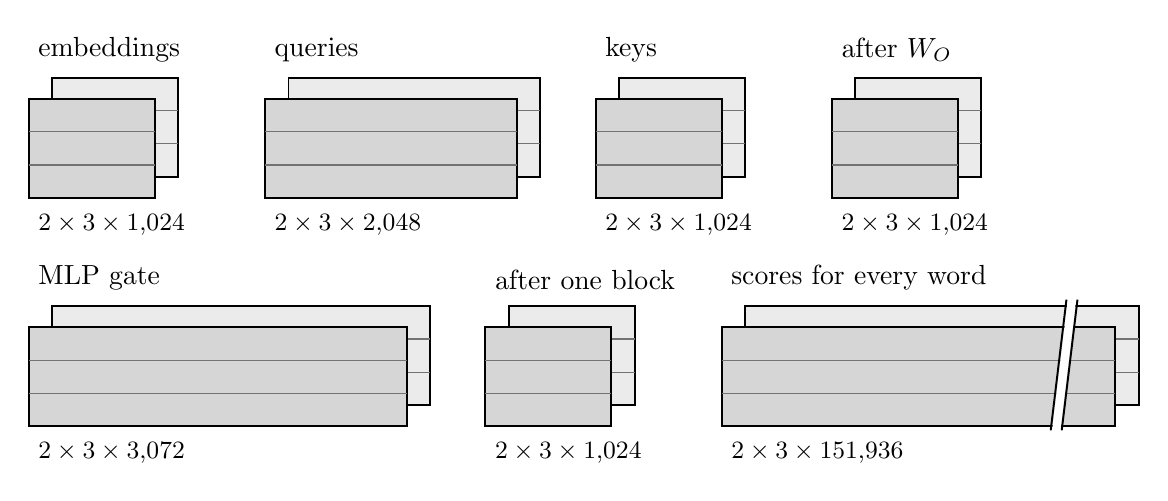
\begin{tikzpicture}
\draw[line width=0.7pt, fill=black!8] (0.300,0.270) rectangle (1.900,-0.990);
\draw[black!55] (0.300,-0.150) -- (1.900,-0.150);
\draw[black!55] (0.300,-0.570) -- (1.900,-0.570);
\draw[line width=0.7pt, fill=black!16] (0.000,0.000) rectangle (1.600,-1.260);
\draw[black!55] (0.000,-0.420) -- (1.600,-0.420);
\draw[black!55] (0.000,-0.840) -- (1.600,-0.840);
\node[anchor=south west, font=\normalsize] at (0.000,0.350) {embeddings};
\node[anchor=north west, font=\small] at (0.000,-1.340) {$2\times3\times1{,}024$};
\draw[line width=0.7pt, fill=black!8] (3.300,0.270) rectangle (6.500,-0.990);
\draw[black!55] (3.300,-0.150) -- (6.500,-0.150);
\draw[black!55] (3.300,-0.570) -- (6.500,-0.570);
\draw[line width=0.7pt, fill=black!16] (3.000,0.000) rectangle (6.200,-1.260);
\draw[black!55] (3.000,-0.420) -- (6.200,-0.420);
\draw[black!55] (3.000,-0.840) -- (6.200,-0.840);
\node[anchor=south west, font=\normalsize] at (3.000,0.350) {queries};
\node[anchor=north west, font=\small] at (3.000,-1.340) {$2\times3\times2{,}048$};
\draw[line width=0.7pt, fill=black!8] (7.500,0.270) rectangle (9.100,-0.990);
\draw[black!55] (7.500,-0.150) -- (9.100,-0.150);
\draw[black!55] (7.500,-0.570) -- (9.100,-0.570);
\draw[line width=0.7pt, fill=black!16] (7.200,0.000) rectangle (8.800,-1.260);
\draw[black!55] (7.200,-0.420) -- (8.800,-0.420);
\draw[black!55] (7.200,-0.840) -- (8.800,-0.840);
\node[anchor=south west, font=\normalsize] at (7.200,0.350) {keys};
\node[anchor=north west, font=\small] at (7.200,-1.340) {$2\times3\times1{,}024$};
\draw[line width=0.7pt, fill=black!8] (10.500,0.270) rectangle (12.100,-0.990);
\draw[black!55] (10.500,-0.150) -- (12.100,-0.150);
\draw[black!55] (10.500,-0.570) -- (12.100,-0.570);
\draw[line width=0.7pt, fill=black!16] (10.200,0.000) rectangle (11.800,-1.260);
\draw[black!55] (10.200,-0.420) -- (11.800,-0.420);
\draw[black!55] (10.200,-0.840) -- (11.800,-0.840);
\node[anchor=south west, font=\normalsize] at (10.200,0.350) {after $W_O$};
\node[anchor=north west, font=\small] at (10.200,-1.340) {$2\times3\times1{,}024$};
\draw[line width=0.7pt, fill=black!8] (0.300,-2.630) rectangle (5.100,-3.890);
\draw[black!55] (0.300,-3.050) -- (5.100,-3.050);
\draw[black!55] (0.300,-3.470) -- (5.100,-3.470);
\draw[line width=0.7pt, fill=black!16] (0.000,-2.900) rectangle (4.800,-4.160);
\draw[black!55] (0.000,-3.320) -- (4.800,-3.320);
\draw[black!55] (0.000,-3.740) -- (4.800,-3.740);
\node[anchor=south west, font=\normalsize] at (0.000,-2.550) {MLP gate};
\node[anchor=north west, font=\small] at (0.000,-4.240) {$2\times3\times3{,}072$};
\draw[line width=0.7pt, fill=black!8] (6.100,-2.630) rectangle (7.700,-3.890);
\draw[black!55] (6.100,-3.050) -- (7.700,-3.050);
\draw[black!55] (6.100,-3.470) -- (7.700,-3.470);
\draw[line width=0.7pt, fill=black!16] (5.800,-2.900) rectangle (7.400,-4.160);
\draw[black!55] (5.800,-3.320) -- (7.400,-3.320);
\draw[black!55] (5.800,-3.740) -- (7.400,-3.740);
\node[anchor=south west, font=\normalsize] at (5.800,-2.550) {after one block};
\node[anchor=north west, font=\small] at (5.800,-4.240) {$2\times3\times1{,}024$};
\draw[line width=0.7pt, fill=black!8] (9.100,-2.630) rectangle (14.100,-3.890);
\draw[black!55] (9.100,-3.050) -- (14.100,-3.050);
\draw[black!55] (9.100,-3.470) -- (14.100,-3.470);
\draw[line width=0.7pt, fill=black!16] (8.800,-2.900) rectangle (13.800,-4.160);
\draw[black!55] (8.800,-3.320) -- (13.800,-3.320);
\draw[black!55] (8.800,-3.740) -- (13.800,-3.740);
\draw[white, line width=3pt] (13.250,-2.550) -- (13.050,-4.210);
\draw[line width=0.7pt] (13.320,-2.550) -- (13.120,-4.210) (13.180,-2.550) -- (12.980,-4.210);
\node[anchor=south west, font=\normalsize] at (8.800,-2.550) {scores for every word};
\node[anchor=north west, font=\small] at (8.800,-4.240) {$2\times3\times151{,}936$};
\end{tikzpicture}}

\caption{The tensors of a real batch inside Qwen3-0.6B, drawn from the recorded shapes. Each sheet is one
sentence ($B=2$), each band one token ($T=3$), and the length is proportional to the width of each token's arrow. The stream (embeddings, after $W_O$, after one block) never changes shape; queries and the MLP
gate are wider; the scores, 151{,}936 per token, are broken off, since at this scale they would be over two
metres long.}
\label{fig:ch10tensors}
\end{figure}

The same shape at pencil size is the batch of Chapter 3: two sentences of three tokens, each token an arrow of
4 numbers. Every tensor in Figure~\ref{fig:ch10tensors} is this, with 1{,}024 (or more) columns instead of 4.

\begin{center}
% AUTO-GENERATED by code/figlib.py helpers -- do not edit
\nTenFit{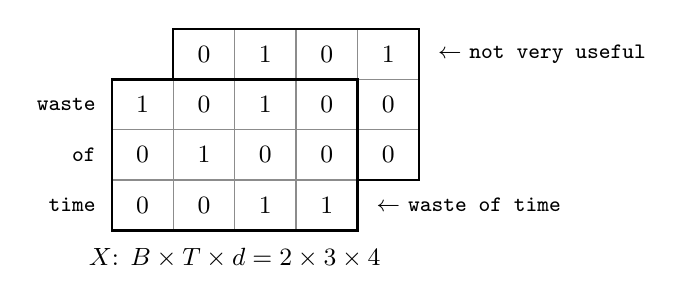
\begin{tikzpicture}
\fill[white] (0.780,0.640) rectangle (3.900,-1.279);
\draw[black!45, fill=white] (0.780,0.640) rectangle (1.560,0.000);
\node[font=\small, text=black] at (1.170,0.320) {$0$};
\draw[black!45, fill=white] (1.560,0.640) rectangle (2.340,0.000);
\node[font=\small, text=black] at (1.950,0.320) {$1$};
\draw[black!45, fill=white] (2.340,0.640) rectangle (3.120,0.000);
\node[font=\small, text=black] at (2.730,0.320) {$0$};
\draw[black!45, fill=white] (3.120,0.640) rectangle (3.900,0.000);
\node[font=\small, text=black] at (3.510,0.320) {$1$};
\draw[black!45, fill=white] (0.780,0.000) rectangle (1.560,-0.640);
\node[font=\small, text=black] at (1.170,-0.320) {$1$};
\draw[black!45, fill=white] (1.560,0.000) rectangle (2.340,-0.640);
\node[font=\small, text=black] at (1.950,-0.320) {$0$};
\draw[black!45, fill=white] (2.340,0.000) rectangle (3.120,-0.640);
\node[font=\small, text=black] at (2.730,-0.320) {$0$};
\draw[black!45, fill=white] (3.120,0.000) rectangle (3.900,-0.640);
\node[font=\small, text=black] at (3.510,-0.320) {$0$};
\draw[black!45, fill=white] (0.780,-0.640) rectangle (1.560,-1.279);
\node[font=\small, text=black] at (1.170,-0.959) {$0$};
\draw[black!45, fill=white] (1.560,-0.640) rectangle (2.340,-1.279);
\node[font=\small, text=black] at (1.950,-0.959) {$0$};
\draw[black!45, fill=white] (2.340,-0.640) rectangle (3.120,-1.279);
\node[font=\small, text=black] at (2.730,-0.959) {$1$};
\draw[black!45, fill=white] (3.120,-0.640) rectangle (3.900,-1.279);
\node[font=\small, text=black] at (3.510,-0.959) {$0$};
\draw[line width=0.9pt] (0.780,0.640) rectangle (3.900,-1.279);
\node[anchor=west, font=\footnotesize] at (4.020,0.320) {$\leftarrow$ \texttt{not very useful}};
\fill[white] (0.000,0.000) rectangle (3.120,-1.919);
\draw[black!45, fill=white] (0.000,0.000) rectangle (0.780,-0.640);
\node[font=\small, text=black] at (0.390,-0.320) {$1$};
\draw[black!45, fill=white] (0.780,0.000) rectangle (1.560,-0.640);
\node[font=\small, text=black] at (1.170,-0.320) {$0$};
\draw[black!45, fill=white] (1.560,0.000) rectangle (2.340,-0.640);
\node[font=\small, text=black] at (1.950,-0.320) {$1$};
\draw[black!45, fill=white] (2.340,0.000) rectangle (3.120,-0.640);
\node[font=\small, text=black] at (2.730,-0.320) {$0$};
\draw[black!45, fill=white] (0.000,-0.640) rectangle (0.780,-1.279);
\node[font=\small, text=black] at (0.390,-0.959) {$0$};
\draw[black!45, fill=white] (0.780,-0.640) rectangle (1.560,-1.279);
\node[font=\small, text=black] at (1.170,-0.959) {$1$};
\draw[black!45, fill=white] (1.560,-0.640) rectangle (2.340,-1.279);
\node[font=\small, text=black] at (1.950,-0.959) {$0$};
\draw[black!45, fill=white] (2.340,-0.640) rectangle (3.120,-1.279);
\node[font=\small, text=black] at (2.730,-0.959) {$0$};
\draw[black!45, fill=white] (0.000,-1.279) rectangle (0.780,-1.919);
\node[font=\small, text=black] at (0.390,-1.599) {$0$};
\draw[black!45, fill=white] (0.780,-1.279) rectangle (1.560,-1.919);
\node[font=\small, text=black] at (1.170,-1.599) {$0$};
\draw[black!45, fill=white] (1.560,-1.279) rectangle (2.340,-1.919);
\node[font=\small, text=black] at (1.950,-1.599) {$1$};
\draw[black!45, fill=white] (2.340,-1.279) rectangle (3.120,-1.919);
\node[font=\small, text=black] at (2.730,-1.599) {$1$};
\draw[line width=0.9pt] (0.000,0.000) rectangle (3.120,-1.919);
\node[anchor=east, font=\footnotesize\ttfamily] at (-0.080,-0.320) {waste};
\node[anchor=east, font=\footnotesize\ttfamily] at (-0.080,-0.959) {of};
\node[anchor=east, font=\footnotesize\ttfamily] at (-0.080,-1.599) {time};
\node[anchor=west, font=\footnotesize] at (3.240,-1.599) {$\leftarrow$ \texttt{waste of time}};
\node[anchor=north, font=\small] at (1.560,-2.019) {$X$: $B\times T\times d = 2\times3\times4$};
\end{tikzpicture}}

\end{center}

\Summary{A real batch keeps the shape $B\times T\times d$ on the residual stream and widens only inside attention,
inside the MLP, and at the final scores.}

%---------------------------------------------------------------------
\subsection*{10.7\quad The arithmetic per token}

\Picture Every parameter in a matrix is used once for every token that passes: one multiplication and one
addition. So the work per token is about twice the number of parameters it passes through.

\Exactly Forward work per token is about $2N$ operations, with $N$ the non-embedding parameters, plus the
attention scores, $2\times\text{layers}\times\text{context}\times\text{heads}\times\text{head width}$ (Kaplan et
al., 2020). Training costs about three times the forward pass (the backward pass of Appendix A does about twice the
forward work), so about $6N$ per token.

\begin{center}
\small
\begin{tabular}{@{}l r r r@{}}
\toprule
model, context & $2N$ part & attention part & forward, per token\\
\midrule
GPT-2 small, 1{,}024 & \nTenGptTwoN\ million & \nTenGptFwdAttn\ million & \nTenGptFwd\ million\\
Qwen3-0.6B, 4{,}096 & \nTenQwenTwoN\ billion & \nTenQwenAttnFour\ billion & \nTenQwenFwdFour\ billion\\
Qwen3-0.6B, 32{,}768 & \nTenQwenTwoN\ billion & \nTenQwenAttnThirtyTwo\ billion & \nTenQwenFwdThirtyTwo\ billion\\
\bottomrule
\end{tabular}
\end{center}

At long context, the attention part overtakes the weights: the price of letting every token look at every earlier
token (Requirement 3 of Chapter 1). And training: $6\times\nTenQwenNonEmbBillions$ billion parameters $\times$
36 trillion tokens $\approx \nTenQwenTrainFlops$ operations.

\begin{checkq}
Doubling the context length of Qwen3-0.6B from 4{,}096 to 8{,}192 tokens roughly does what to the forward work per
token?
\begin{options}
\item Doubles all of it.
\item Leaves the $2N$ part unchanged and doubles the attention part.
\item Leaves it unchanged; work depends only on parameters.
\item Quadruples all of it, because attention is quadratic.
\end{options}
\end{checkq}

\Summary{Per token, forward work is about twice the non-embedding parameters plus an attention term that grows with
context; training is about three times that.}

%---------------------------------------------------------------------
\subsection*{10.8\quad Line by line: toy, GPT-2, Qwen3}

\begin{center}
\footnotesize
\begin{longtable}{@{}P{2.3cm} P{2.7cm} P{3.3cm} P{3.4cm} P{2.4cm}@{}}
\toprule
component & toy & GPT-2 small (2019) & Qwen3-0.6B (2025) & why it changed\\
\midrule
\endhead
tokenizer & whole words, 12 & byte-level BPE, 50{,}257 & byte-level BPE, 151{,}936 rows & Ch.\ 2: no unknown words; more languages need more tokens\\
embeddings & $12\times4$ table & $50{,}257\times768$ & $151{,}936\times1{,}024$ & Ch.\ 2\\
positions & none (order lost, \S3.11) & learned table, 1{,}024 slots & RoPE rotation, no parameters & Ch.\ 4: relative positions, longer contexts\\
norm & none & LayerNorm before each sublayer & RMSNorm before each sublayer, plus QK-norm & Ch.\ 6: stable depth; \S10.3\\
attention & 1 head of 4 & 12 heads of 64 & 16 query heads of 128, 8 key-value heads & Ch.\ 5, Ch.\ 9: cache bill\\
MLP & --- & GELU, $768\to3{,}072\to768$ & SwiGLU, gate and up $1{,}024\to3{,}072$, down & Ch.\ 5\\
biases & none & on every linear map & none & dropped in Qwen3 (Yang et al., 2025)\\
residual stream & --- & yes & yes & Ch.\ 5\\
final norm & --- & LayerNorm & RMSNorm & Ch.\ 6\\
unembedding & --- & tied to embeddings & tied to embeddings & Ch.\ 7\\
\bottomrule
\end{longtable}
\end{center}

\begin{breaks}
This table compares two published designs. It does not tell you that each change made the model better on its
own; the reports describe what was built, and only some changes were tested one at a time. Chapter 11 shows how to
test a change yourself.
\end{breaks}

\begin{principle}{read the configuration, not the name}
A model's name gives one rounded number. Its configuration gives every shape, and from the shapes you can derive
the parameter count, the arithmetic per token, the memory per token of conversation (Chapter 9) and where each
cost comes from. The same habit pays off in any system you build or buy: an agent's tool list, a memory
store's schema, a pipeline's config file. Derive the costs from the declared shapes, then check your derivation
against the running system. When the two disagree, the disagreement shows you where your understanding was wrong.
\end{principle}

\begin{lookingback}
\begin{enumerate}[label=\arabic*.,leftmargin=1.6em]
\item (Chapter 3) Why did we divide scores by $\sqrt{d_k}$? With Qwen3's head width of 128, what is the divisor?
\item (Chapter 9) Using Qwen3's configuration, recompute its cache per token.
\item (Chapter 1) Which of the four requirements of Chapter 1 does each of these meet: embeddings, RoPE,
attention, the causal mask?
\end{enumerate}
\end{lookingback}

%---------------------------------------------------------------------
\subsection*{Exercises}

\begin{exercise}
Recount GPT-2 small's attention parameters per block from the shapes: $W_{QKV}$ is $768\times2{,}304$ with 2{,}304
biases, and $W_O$ is $768\times768$ with 768 biases. Check your answer against the table.
\end{exercise}

\begin{exercise}
(Fading.) Fill in the Qwen3 MLP count: gate $1{,}024\times\underline{\quad}$, up $1{,}024\times\underline{\quad}$,
down $\underline{\quad}\times1{,}024$; total \underline{\quad}.
\end{exercise}

\begin{exercise}
Suppose Qwen3-0.6B did \emph{not} tie its unembedding to its embedding table. How many parameters would it have,
and what share of them would be the two tables together?
\end{exercise}

\begin{exercise}
Design question. You must halve Qwen3-0.6B's cache per token without changing its width or number of layers. Name two
configuration changes that do it, and for each, say what you expect to lose.
\end{exercise}

%---------------------------------------------------------------------
\subsection*{Answers to Chapter 10}

\paragraph{Check yourself 10.1.} (b). The 16 query heads produce 2{,}048 numbers, and $W_O$ maps them back to the stream
width 1{,}024. (a) is misconception M10.6. (c) has the direction reversed. (d) forgets that heads' outputs must be
brought back to width $d$ before being added to the residual stream (Chapter 5).

\paragraph{Check yourself 10.2.} (b). The $2N$ part depends only on the parameters; the attention part is proportional
to context. (a) treats all work as attention. (c) ignores the scores. (d) confuses the work for one new token with the
work for the whole sequence, which does grow quadratically.

\paragraph{Looking back.} (1) To keep random scores about one unit wide at any head width, so softmax does not start
saturated (\S3.8); $\sqrt{128}\approx11.3$. (2) $2\times28\times8\times128\times2 = \nNineQwenPerTok$ bytes. (3) Embeddings
meet Requirement 1 (similarity), RoPE Requirement 2 (order), attention Requirement 3 (direct reach) and, with the mask,
Requirement 4 (all positions at once, honestly).

\paragraph{Exercise 10.1.} $768\times2{,}304 + 2{,}304 + 768\times768 + 768 = \nTenGptAttn$, as in the table.

\paragraph{Exercise 10.2.} 3{,}072, 3{,}072, 3{,}072; $3\times1{,}024\times3{,}072 = \nTenQwenMlp$.

\paragraph{Exercise 10.3.} Add another $151{,}936\times1{,}024 = \nTenQwenEmbed$: \nTenQwenUntied\ parameters, of which
\nTenQwenUntiedShare\% would be the two tables.

\paragraph{Exercise 10.4.} Halve the key-value heads (8 to 4): fewer independent ways to describe each token. Or halve the
head width (128 to 64) for keys and values: each key and value carries fewer numbers. A third option, storing the cache
in 8 bits instead of 16, changes no configuration number but loses precision.

\subsection*{What you now know}
\begin{itemize}
\item How to read a configuration and derive every shape in the model from it.
\item How to count parameters by component; the counts match the real models exactly
(\nTenGptTotal\ and \nTenQwenTotal).
\item That most parameters live in the MLPs and the embedding table, not in attention.
\item What changed from the toy to GPT-2 to Qwen3, and which chapter motivates each change.
\item That forward work is about $2N$ per token plus an attention term that grows with context, and training about $6N$.
\end{itemize}
